\chapter{\texorpdfstring{Search for New Physics in $\tau^+\tau^-\tau^+\tau^-$ Final States}{Search for new physics in tautautautau final states}}
\label{sec:H_A_to_4_tau_analysis}

Enhancement from $\tan\beta$ to up or down-like quark couplings to additional Higgs bosons are essential for the majority of searches for extended Higgs sectors, including in the analysis detailed in Chapter~\ref{sec:bsm_H_to_tau_tau_analysis}.
However, in some 2HDMs it can be the case that both up and down-like couplings to additional Higgs bosons are suppressed and this parameter space is left relatively untouched by "MSSM-like" searches.
In particular, type X 2HDMs where only lepton couplings are enhanced by $\tan\beta$, allow for new physics loop contributions to SM measurements through couplings between leptons and additional Higgs bosons.
This is particularly interesting in the context of the g-2 anomaly \cite{} with reasoning explained in Section~\ref{}.
This chapter will detail a search for such an extended Higgs sector, that looks for a production mode not suppressed at high $\tan\beta$, through the process $Z^{*}\rightarrow \phi A \rightarrow 4\tau$.
This search is split up into two sections:

\begin{enumerate}[i)]
  \item A model independent search for the $Z^{*}\rightarrow \phi A \rightarrow 4\tau$ process. Both additional particles are required to have narrow width and no assumptions are made on the production cross-section via an off-shell Z boson or the branching fraction of $phi$ and A decaying to a pair of tau leptons.
   \item A search for the type X 2HDM, motivated by the phase space for possible explanations to the g-2 anomaly. The $m_{A}$-$\tan\beta$ phase space for scenarios of $m_\phi$ in the alignment limit is scanned, as well as checks outside of this limit on the $\cos(\beta-\alpha)$-$\tan\beta$ for specific scenarios of both $m_\phi$ and $m_A$.
\end{enumerate}

These searches are performed with the full run-2 dataset ($138 \sifb$) collected by the CMS experiment. 

\section{Signal Modelling}

Any additional Higgs boson produced in the type X 2HDM at high $\tan\beta$ will predominantly decay to tau leptons.
To probe the type X 2HDM at high $\tan\beta$, a production process that is not suppressed is required.
Ref.~\cite{Jueid:2021avn} discusses that the following production modes of two additional Higgs bosons are dominant to produce any of these new particles at high $\tan\beta$:
\begin{enumerate}[i)]
  \item $pp \rightarrow Z^{*} \rightarrow \phi A \rightarrow (\tau^{-}\tau^{+})(\tau^{-}\tau^{+})$
  \item $pp \rightarrow Z^{*} \rightarrow H^{+}H^{-} \rightarrow (\tau^{-}\nu)(\tau^{+}\nu)$
  \item $pp \rightarrow W^{\pm *} \rightarrow H^{\pm}A \rightarrow (\tau^{\pm}\nu)(\tau^{-}\tau^{+})$
  \item $pp \rightarrow W^{\pm *} \rightarrow H^{\pm}\phi \rightarrow (\tau^{\pm}\nu)(\tau^{-}\tau^{+})$
\end{enumerate}
As the production cross sections are of the similar magnitudes, the search sensitivities depend on the separation of the signals from background.
In general, the more objects you can select in the final state, the smaller the background contributions.
This is certainly true in tau enriched final states, where backgrounds can be dominated jets misidentified as hadronic taus and so every extra tau selected reduces this background.
In particular, (ii) has the production cross sections \cite{} far smaller than the observed limit for gluon fusion production of a single resonance shown in Figure~\ref{fig:model_independent_limits}(a) and it is not possible to use tau decay product and MET alignment to separate the background, so does seem not a viable search option with the run-2 CMS dataset.
The increased background from fewer object selections and looser charge sum selection on (iii) and (iv), makes (i) the golden search channel for a type X 2HDM. 
A Feynman diagram for this process is shown in Figure~\ref{fig:4tau_feynamn}. \\

\begin{figure}[H]
\centering
\begin{tikzpicture}[scale=2]
  \begin{feynman}
    \vertex [label=left:$q$] (a1) at (0,-0.25);
    \vertex [label=left:$\bar{q}$] (a2) at (0,1.25);
    \vertex (b) at (0.7,0.5);
    \vertex [label=above:$Z^{*}$] (b1) at (1.05,0.5);    
    \vertex (c) at (1.4,0.5);
    \vertex [label=below:$h/H$] (d11) at (1.75,0.15);
    \vertex [label=above:$A$] (d12) at (1.75,0.85);
    \vertex (d1) at (2.1,0);
    \vertex (d2) at (2.1,1);
    \vertex [label=right:$\tau^-$] (e1) at (2.7,-0.25);
    \vertex [label=right:$\tau^+$] (e2) at (2.7,0.25);
    \vertex [label=right:$\tau^-$] (e3) at (2.7,0.75);
    \vertex [label=right:$\tau^+$] (e4) at (2.7,1.25);
    \diagram* {
      (a1) -- [fermion] (b),
      (b) -- [fermion] (a2),
      (b) -- [photon] (c),
      (c) -- [scalar] (d1),
      (c) -- [scalar] (d2),
      (d1) -- [fermion] (e1),
      (e2) -- [fermion] (d1),
      (d2) -- [fermion] (e3),
      (e4) -- [fermion] (d2),
    };
  \end{feynman}
\end{tikzpicture}
\vspace*{10mm}
\caption{Diagram of production of two additional neutral Higgs bosons from an off-shell Z boson and their decays to tau leptons.}
\label{fig:4tau_feynamn}
\end{figure}

Signal templates for the production of this process with a mass grid for $\phi$ and A between 100 to 300 and 60 to 160 GeV respectively are generated.
These mass ranges are motivated from the results in Table~\ref{tab:gm2region}.
The samples are simulated in the five-flavour scheme (5FS) at NLO precision using the \MGvATNLO v2.6.5 event generator~\cite{Alwall:2011uj}.
Generation is performed using the parton distribution function (PDF) NNPDF3.1~\cite{Ball:2014uwa,Ball:2017nwa}, where $\tau$ lepton decay, parton showering and hadronisation are all modelled with the \PYTHIA event generator with the PU profile matched to data~\cite{Sirunyan:2019dfx,Sjostrand:2014zea}.
The events are then passed through the \texttt{GEANT4}-based \cite{Agostinelli:2002hh} simulation of the CMS detector and reconstructed in the same way as data.
Generator level distributions of di-$\tau$ mass distributions from the decay of $\phi$ and A are shown in Figure~\ref{}.\\

FIGURE OF GENERATOR LEVEL MASSES \\

The cross sections in the alignment scenarios are also determined with this procedure and vary from 10 fb (highest $m_{A}$ and $m_{\phi}$ scenario) to 650 fb (lowest $m_{A}$ and $m_{\phi}$ scenario), as shown in Figure~\ref{fig:4tau_xs}.
These are independent of $\tan\beta$, however, out of the alignment scenarios the cross sections for H scales with $\sin^{2}(\beta-\alpha)$ and h scales with $\cos^{2}(\beta-\alpha)$.

\begin{figure}[!hbtp]
\centering
    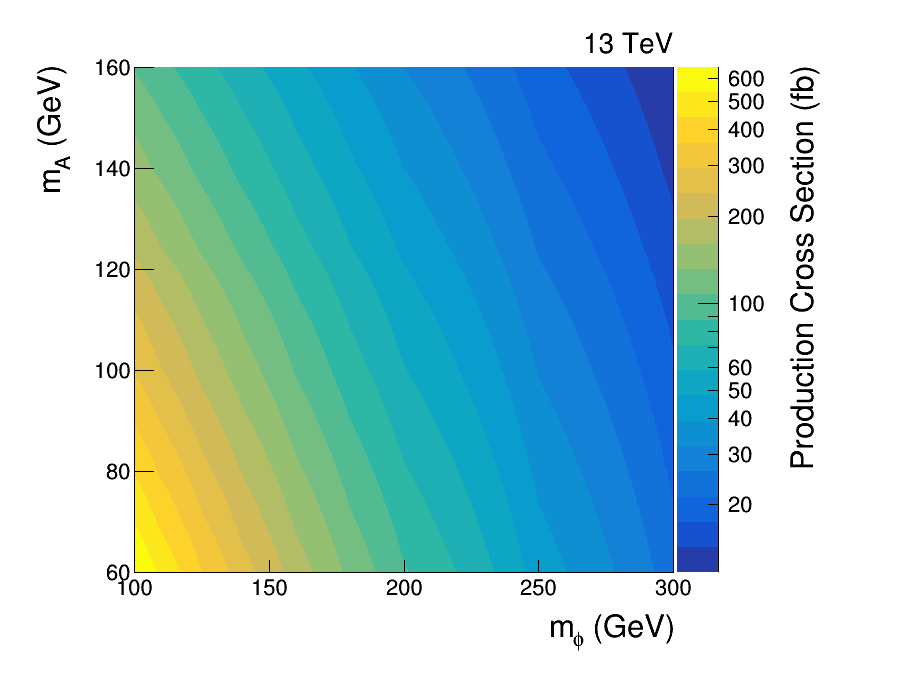
\includegraphics[width=0.8\textwidth]{Figures/cross_sections.png}
\caption{Calculated productions cross sections for the $Z^{*} \rightarrow \phi A$ process, varying the masses of $\phi$ and A.}
\label{fig:4tau_xs}
\end{figure}

The branching fractions of $\phi$ and A to pairs of $\tau$ leptons is dependent on both $tan\beta$ and $\beta-\alpha$.
For this analysis, the branching fractions are calculated using \texttt{2HDECAY} \cite{Krause:2018wmo}.
In the alignment scenarios, the $A\rightarrow\tau\tau$ branching fractions are approximately 1 above $\tan\beta \approx 2$, where below they sharply drop off and other processes such as $A\rightarrow b\bar{b}$ become dominant.
This is also true for $\phi\rightarrow\tau\tau$ branching fractions, except in the case where $m_\phi$ is greater than $m_A$ by more than $m_Z$ and so the $\phi\rightarrow ZA$ decay becomes kinematically feasible and can dominate at high $\tan\beta$.
Examples of this are shown in Figure~\ref{fig:4tau_br_1d}.
Out of the alignment scenario, the branching fractions of $\phi$ to tau leptons becomes smaller as the magnitude of the coupling of additional neutral Higgs bosons to taus is reduced, whilst the $A$ branching fractions, like the couplings, are left unchanged.
An example of the $\phi$ branching fractions out of the alignment scenario is shown in Figure~\ref{fig:4tau_br_2d}.

\begin{figure}[!hbtp]
\centering
    \subfloat[]{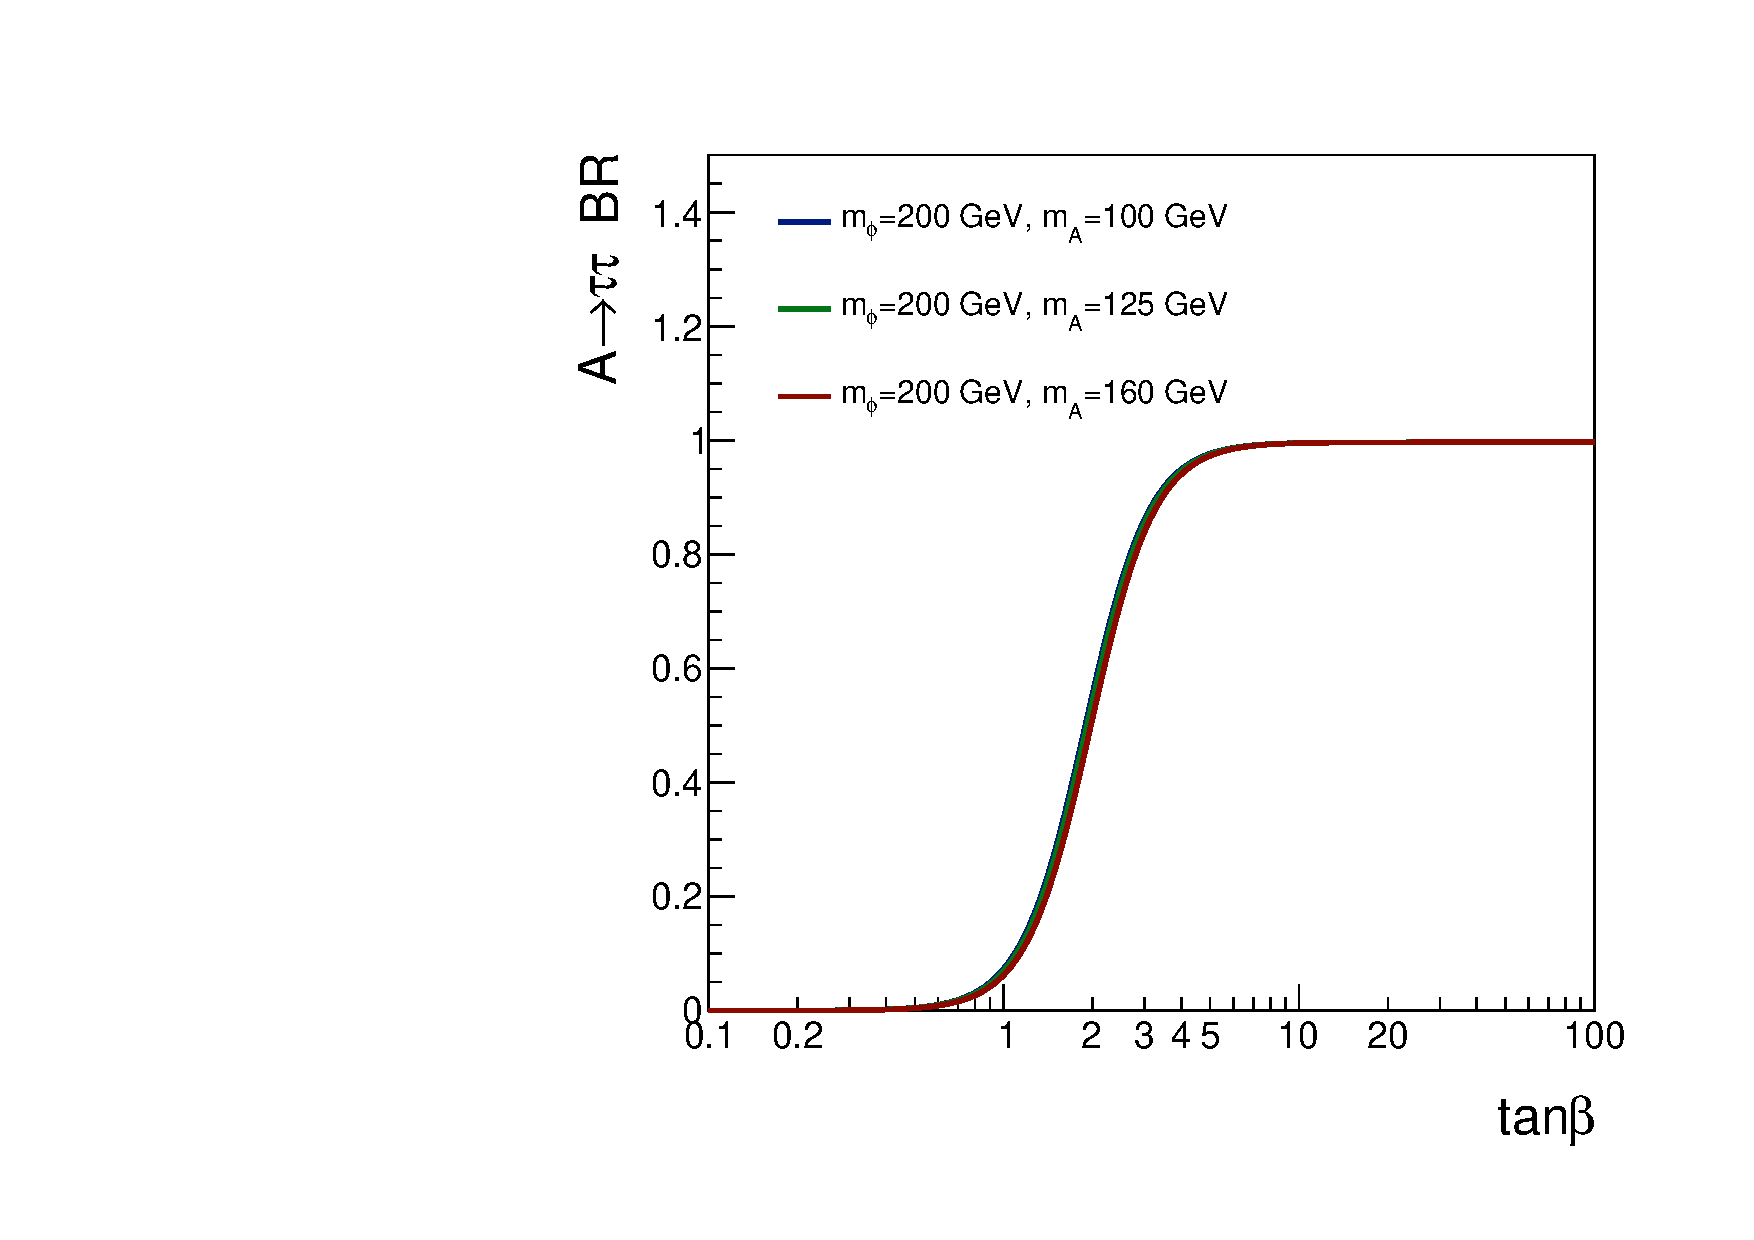
\includegraphics[width=0.45\textwidth]{Figures/A_br_plot_mphi200.pdf}}
    \subfloat[]{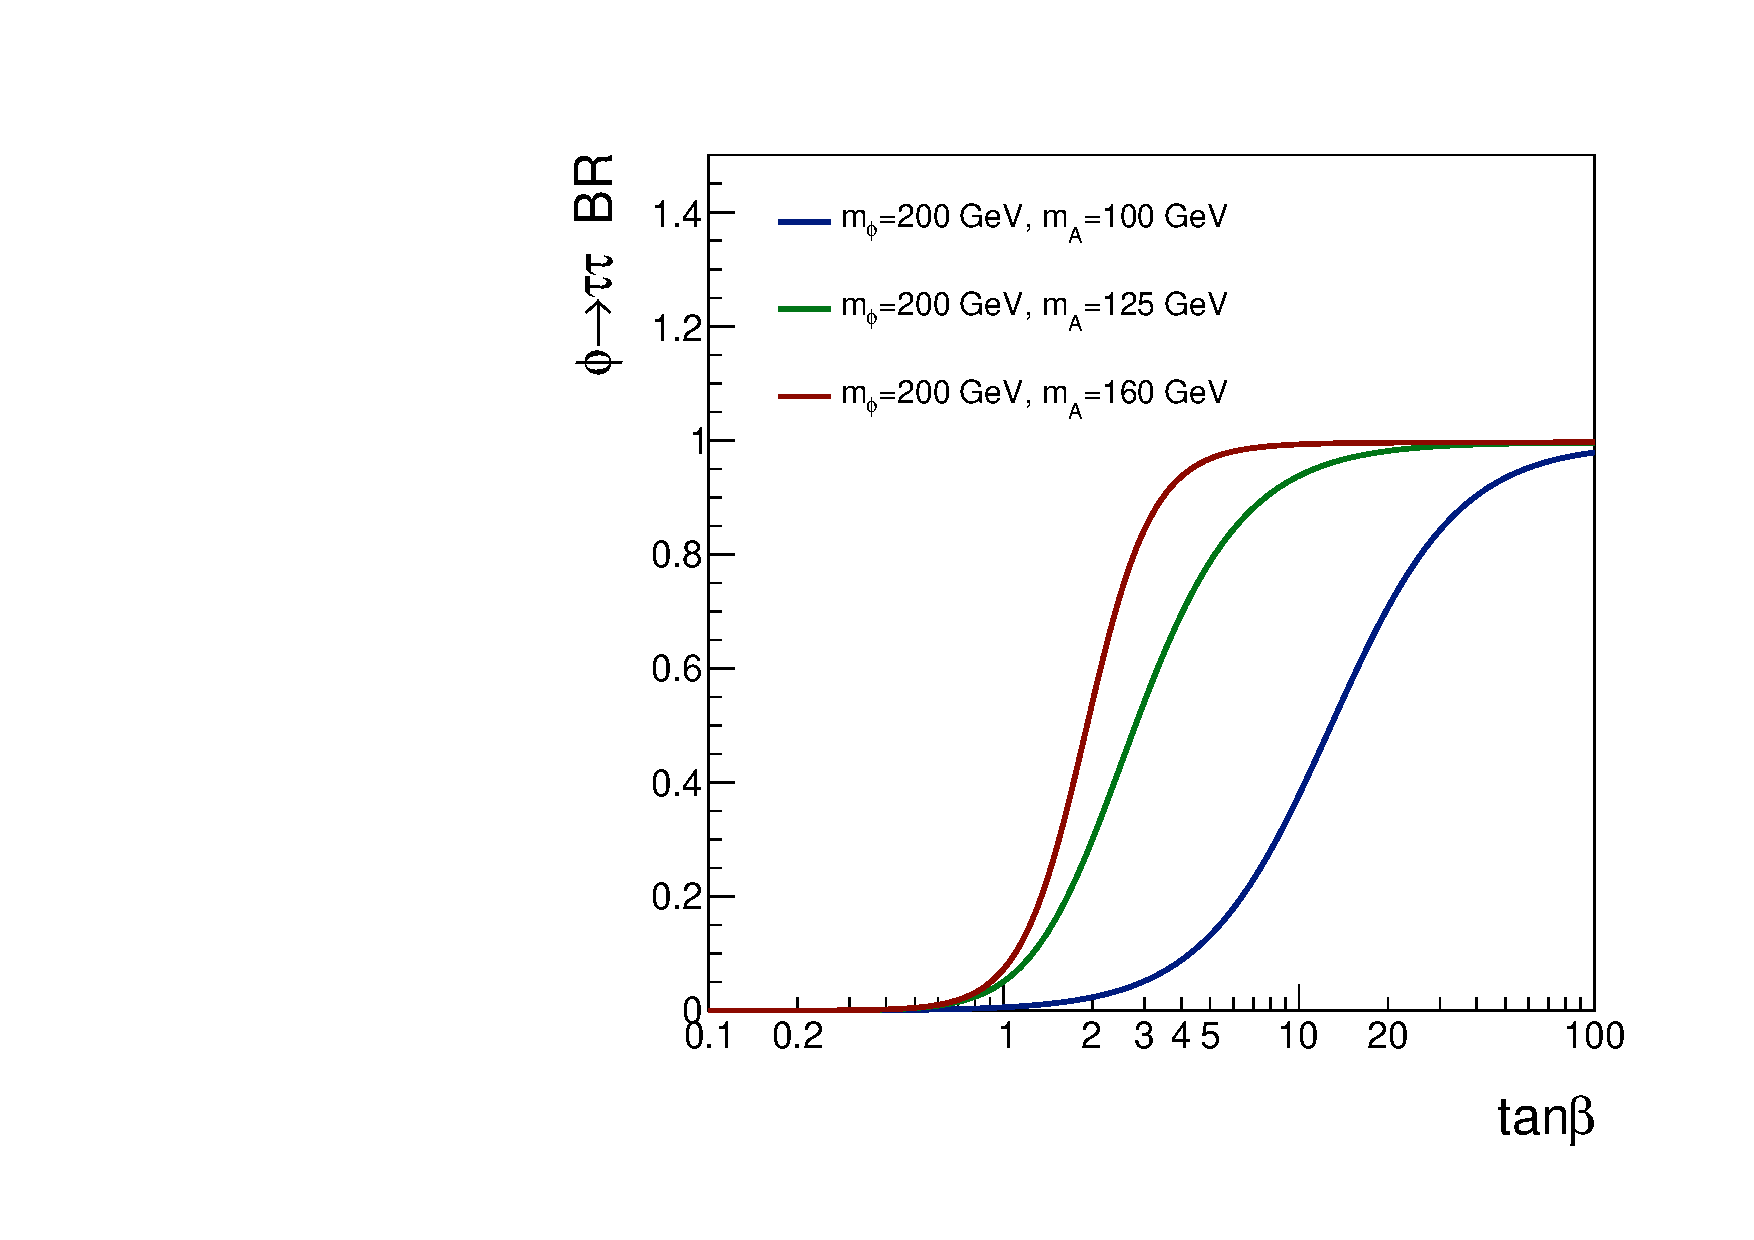
\includegraphics[width=0.45\textwidth]{Figures/phi_br_plot_mphi200.pdf}} 
\caption{Calculated branching fractions of A (a) and $\phi$ (b) decaying to a pair of $\tau$ leptons for various mass scenarios.}
\label{fig:4tau_br_1d}
\end{figure}

\begin{figure}[!hbtp]
\centering
    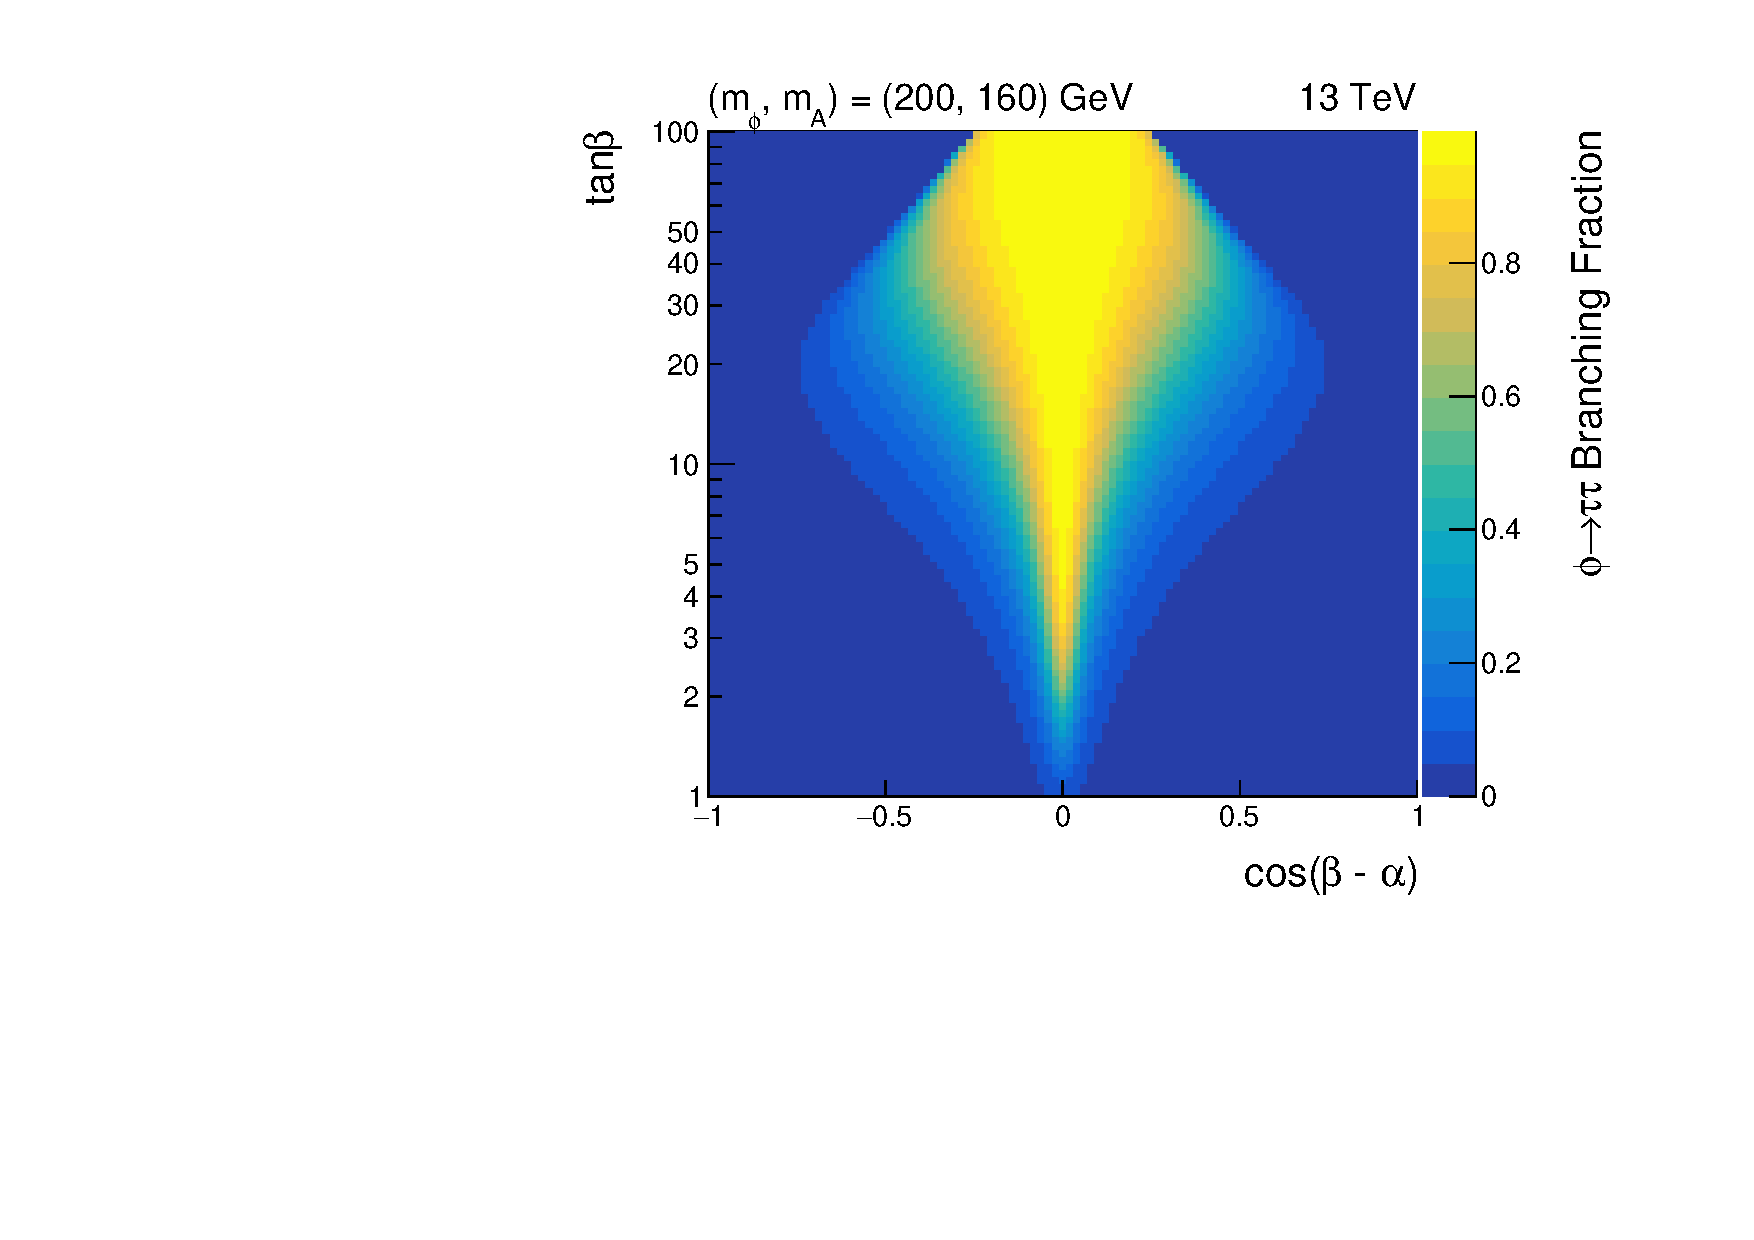
\includegraphics[width=0.7\textwidth]{Figures/phi_branching_fractions_mphi200_mA160.pdf}
\caption{Calculated branching fractions in the $\cos(\beta-\alpha)$-$\tan\beta$ phase space for $\phi$ of mass 200 GeV decaying to a pair of $\tau$ leptons, in the scenario where $m_A = 160$ GeV.}
\label{fig:4tau_br_2d}
\end{figure}

\section{Event Selection}

In comparison to Chapter~\ref{sec:bsm_H_to_tau_tau_analysis}, four $\tau$ leptons produce a much larger number of possible final states. 
All possible variation of e, $\mu$ and $\tau_h$ final state combinations and their branching fractions are shown in Table~\ref{tab:4tau_bf}.
Just under 90\% of the branching ratio goes to decay products containing two or more hadronic taus.
These are the main final states that are explored in this analysis. 
In addition to this, an orthogonal $\tau_h \tau_h \tau_h$ channel is added to target events where reconstruction of the $\tau_h \tau_h \tau_h \tau_h$ channel loses a single $\tau_h$ object.
This can come about due to low triggering and ID efficiency of $\tau_h$ candidates, as well as the high $\pT$ thresholds required for both. \\

\begin{table}[H]
    \centering
    \begin{tabular}{|c|c|}
         \hline
         Channel & Branching Fraction  \\
         \hline
         \hline
         $e \tau_h \tau_h \tau_h$ & 19.4\% \\
         $\mu \tau_h \tau_h \tau_h$ & 18.9\% \\
         $\tau_h \tau_h \tau_h \tau_h$ & 17.6\% \\
         $e \mu \tau_h \tau_h$ & 15.6\% \\
         $e e \tau_h \tau_h$ & 8.0\% \\
         $\mu \mu \tau_h \tau_h$ & 7.6\% \\
         $e e \mu \tau_h$ & 4.3\% \\
         $e \mu \mu \tau_h$ & 4.2\% \\
         $e e e \tau_h$ & 1.5\% \\
         $\mu \mu \mu \tau_h$ & 1.4\% \\
         $e e e \mu$ & 1.4\% \\
         $e e \mu \mu$ & 0.6\% \\
         $e \mu \mu \mu$ & 0.4\% \\
         $e e e e$ & 0.1\% \\
         $\mu \mu \mu \mu$ & 0.1\% \\
         \hline
    \end{tabular}
    \caption{}
    \label{tab:4tau_bf} 
\end{table}

\subsection{Trigger Requirements}

Given that each final state is not exactly triggered on, there is no obvious choice for what triggers to use. 
A variety of triggers are available for individual and clusters of objects in the final state. 
The possible triggers for single objects are the SingleElectron and SingleMuon triggers. 
This is not the case for the SingleTau trigger as it has a $\pT$ threshold too high for it to be useful. 
The possible triggers for clusters of objects are the DoubleElectron, DoubleMuon, DoubleTau, Electon-Muon cross, Muon-Tau cross and Electron-Tau cross. 
The $\pT$ thresolds of the mentioned triggers are shown in Table~\ref{tab:trig_thres} and the corresponding HLT paths used for each year are shown in Tables~\ref{tab:HLTPaths2016}-\ref{tab:HLTPaths2018}.

The decision on which trigger to use is a balance between simplicity, due to the corrections that need to be applied, and trigger acceptance. 
The trigger acceptance of a number of trigger combinations in a number of different channels were calculated and shown in Table~\ref{tab:trigeff}. 
Firstly, the SingleElectron and SingleMuon triggers were chosen for the signal acceptance table over the DoubleElectron and DoubleMuon triggers in the $ee\tau_h \tau_h$, $\mu\mu\tau_h \tau_h$. 
This is motivated by the lack of sensitivity we expect to have in these channels, as they have the small branching fractions, and backgrounds from Z + 2 jet fakes and ZZ events including leptons would be larger than in other channels. 
Using the single triggers in this channels would allow them to be more consistent with other more sensitive channels including leptons and correlate relevant trigger uncertainties.



\subsection{Offline Requirements}

Deeptau working points

On top of the object selection, there are few further selections on the total tau collection.

\textbf{Charge}~\\
As the two tau pairs from the signals originate from two neutral additional Higgs bosons, the sum of charge of the fully reconstructred objects should be 0. This is applied in the decay channels where there are four objects. In the $\tau_h \tau_h \tau_h$ the assumption is that a hadronic tau has been lost, so the charge selection required here is that the absolute value of the sum of the charges of the object must be 1.

\textbf{Event Vetos}~\\
In order to ensure the orthogonality between channels, a number of vetos are needed. The constraints set on the number of leptons for each channel are shown in Table~\ref{tab:leptonvetoes}.

\begin{itemize}
  \item Extra Lepton Veto
  \begin{itemize}
    \item Extra lepton vetos are used in all decay channels.
    \item Orthogonality is achieved by requiring the absence of additional electrons and muons on top of those already part of the selected pair.
    \item The kinematic requirements, ID and isolation requirements on these extra leptons are at least as loose as the loosest cuts required for signal electron or muon of the final states.
  \end{itemize}
  \item Extra Hadronic Tau Veto
  \begin{itemize}
    \item The $\tau_h \tau_h \tau_h \tau_h$ and $\tau_h \tau_h \tau_h$ are the only channels now not orthogonal after extra lepton vetos.
    \item In the $\tau_h \tau_h \tau_h$ channel, any extra hadronic tau candidate passing the signal selection is vetoed.
  \end{itemize}
\end{itemize}


\section{Search Optimisation}

TALK ABOUT CATEGORY OPTIMISATION \\

\begin{figure}[!hbtp]
\centering
    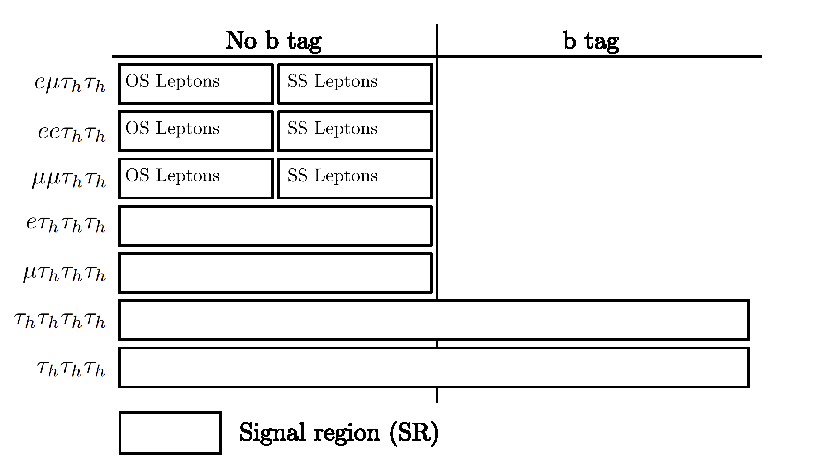
\includegraphics[width=0.85\textwidth]{Figures/event-categories_4tau.pdf}
\caption{Overview of the categories used for the extraction of the signal in the $Z^{*}\rightarrow \phi A \rightarrow 4\tau$.}
\label{fig:high_mass_categories}
\end{figure}

The variable $m_{T}^{\text{tot}}$ is defined as:
\begin{equation}
m_{T}^{\text{tot}} = \sqrt{ \sum_{i=1}^{N_\tau} m_{T}(\vec{p}_{T}^{\hspace{2pt}\tau_i},\vec{p}_{T}^{\hspace{2pt}\text{miss}})^2 + \sum_{i,j=1; i \neq j}^{N_\tau} m_{T}(\hspace{2pt}\vec{p}_{T}^{\tau_i},\hspace{2pt}\vec{p}_{T}^{\tau_j})^2 },  
\end{equation}
 
\section{Background Modelling Overview}

The background is split into two components in each decay channel. These are events where at least one hadronic tau is a jet fake and the remaining contribution dominated by events where all objects are correctly selected. The former is derived using a machine learning fake factor approach as described in Section~\ref{subsec:ff} and the latter is modelled by MC and modelling checked with a control region as described in Section~\ref{subsec:genuinetau}.



\section{ZZ Modelling}
\section{Machine Learning Fake Factor Method}
\subsection{BDT Reweighter}

Ref.~\cite{Rogozhnikov:2016bdp} proposes a new method utilising machine learning techniques to solve the issues with the previous approach. It looks to optimise the regions that most need reweighting. A good way to do this is using a decision tree, as with this the data can be split into "leafs" by checking simple conditions. To best choose the regions that need reweighting the algorithm looks to maximise the symmetrised $\chi^2$.

\begin{equation}
\chi^2 = \sum_{\text{leaf}} \frac{(w_{\text{leaf, 1}}-w_{\text{leaf, 2}})^2}{(w_{\text{leaf, 1}}+w_{\text{leaf, 2}})^2}
\end{equation}

The larger the value of $\chi^2$ the more important reweighting is in this region. The kind of tree is utilised many times in the reweighting algorithm shown below:

\begin{enumerate}
\item Input training dataset with a large number of variables.
\item Build a tree as stated above. If not the first loop, use newly determined weights.
\item Compute predictions in the leaves $r_{\text{leaf}} = \log\frac{w_{\text{leaf, 1}}}{w_{\text{leaf, 2}}}$. The logarithm is taken so weights in different trees can be summed as usually done in boosting.
\item In each leaf MC events by $w = w \times e^{r_{\text{leaf}}}$.
\end{enumerate}

The final two steps are identical to the first approach except for the use of the logarithm for convenience using boosting. The major difference being how the bins used for reweighting are found, and that this step is repeated multiple times.

\subsection{Fitting Regions}

Unlike the standard fake factor method, statistics are not a problem using the BDT reweighter when choosing which variables you can use to parameterise the fake rate. Therefore rather than fitting two fake factor regions separately and then a correction from sideband to signal to account for missing parameterisation, we can fit the fake rate in regions B,C and D from Figure~\ref{fig:ff_diagram} simultaneously to improve statisitics. \\

The variable used for the sideband variable where we have four objects is whether the total charge is 0 or not. In the $\tau_h \tau_h \tau_h$ channel this is whether the absolute value of the total charge is 1 or not. More than one alternative sideband variables are used in this analysis, this matches what is done for the di-tau fully hadronic fake factors, using whether other hadronic taus (that you are not fitting the fake rate for) pass or fail the tau ID. The split is defined as whether all hadronic taus pass the tau ID and where one or more taus fail the tau ID. \\

Every hadronic tau in the event is treated as a separate entry in the BDT reweighter. As the Loose DeepTauVsJets working point is used for the tau ID, an additional looser baseline selection of rawDeepTauVsJetsScore $\geq$ 0.1 for each hadronic tau is applied to keep the fail and pass tau ID regions not too far separated from one another. Each channel is fitted separately but all years are combined into a single fit. \\

Using this method for deriving the regions used for fitting there would be some overlap in the $\tau_h \tau_h \tau_h \tau_h$ channel with the $\tau_h \tau_h \tau_h$ signal region. As this region is expected to be sensitive to signal this is not used to model jet fakes background. Instead the fake factors for the $\tau_h \tau_h \tau_h \tau_h$, use the fit from the $\tau_h \tau_h \tau_h$ channel. There are a few variables that are defined differently in the fit between the two channels due to the difference of 4 to 3 objects selected, therefore when getting fake factors in the $\tau_h \tau_h \tau_h \tau_h$, the lowest DeepTauVsJets scoring unused hadronic tau candidate is dropped and variables recalculated. This candidate is chosen to be removed to best mimic the initial selection of the hadronic tau candidates where they are sorted by DeepTauVsJets score and the high scoring candidates are chosen. As shown later in this section, there is no major dependence on the shifted variables and any effect from this removal is covered within the uncertainty model. \\

After this looser baseline tau ID is applied, following the logic stated above the below regions are reweighted onto one another to provide the fake factors. Each hadronic tau is labelled numerically and whether it passes the Loose WP of hadronic tau $i$ as $P_{i}$. The total bracket with its index shown, means the features of that hadronic tau is used. \\

\subsection{Machine Learning Subtraction Method}

In the standard fake factor method, histograms are used to fit the fake factors rather than datasets. 
Using histograms, the small fraction of events which are not jet fakes can easily be subtracted off. 
To do this, the data histogram is subtracted from by a stacked MC background produced with generator matching ensuring the event is not a jet fake and this produces a data-MC hybrid histogram of predicted jet fake events.
However, subtraction is not possible with a full dataset and negative weights do not work with the BDT reweighter. 
Therefore, the only option is to remove like-for-like events in data compared to the non jet fake generator matched MC.
An example of this is template matching, which takes an event and can find the closest event in another datasets.
But as the fitting dataset is highly dimensional, this requires too much computation.
The solution proposed for this is to use a BDT to reduce the dimensionality of the datasets effectively the one dimension of an output score of a simple binary classifier.

\begin{itemize} 
  \item In each channel, all MC in the fitting region is stacked and scaled to cross section (via weighting) and the variables used for reweighting (Section~\ref{sec:var_for_reweighting}) are put into a dataset.
  \item Events that are jet fakes and not jet fakes are separated into the two classes that will be used for the binary classification.
  \item To ensure unbiased training, the weights of the two categories are normallised to one another.
  \item A BDT is then trained to separate whether the MC is jet fake or not.
  \item The scores of the BDT for how likely the event is not a jet fake is added to the dataset.
  \item The scores of the non jet fake events are drawn into a histogram with a number of bins suitable for the number of statistics and rescaled to cross section to best match what would be observed in data.
  \item The output score of the BDT is added to data events
  \item Each bin of the MC histogram is then looped through:
  \begin{itemize}
    \item Data events with BDT score within the range of the bin are selected.
    \item Events within this bin are then randomly sample and removed.
    \item This stops when the number of events removed equals to the number of non jet fake events predicted in the MC histogram bin.
  \end{itemize}
\end{itemize}

This method then gives a data-MC hybrid method to determine a dataset of predicted jet fake events and should given near identical results when drawing out histograms in all variables compared to subtracting off MC non jet fakes events from a data histogram as used in the original fake factor method.
It allows for non jet fake-like events to be sampled and removed to the correct yield through all variables.
It is important to remove events throughout the MC non jet fake BDT score histogram as if only the highest score events were removed, these events would come primarily from the tails of the distribution where it is easiest to separate jet fake and non jet fakes.
To validate this method, histograms are shown in Figures~\ref{fig:ff_sub_ttt}--\ref{fig:ff_sub_emtt}, comparing the BDT subtraction method and histogram subtraction method for a few of the fitted variables.

\subsection{Fitting}

The variables used to fit the BDT reweighter on the subtracted datasets are variables that have been shown to have fake rate dependence previously. Also added are the variables that take you from B to A and C to A, from Figure~\ref{fig:ff_diagram}. As all years are fit together, in order to account for any differences in fake rate from year to year, this is also added. All these variables are shown below.

\begin{itemize}
\item The HPS decay mode of the hadronic tau candidate.
\item $\pT$ of the hadronic tau candidate.
\item The ratio of the $\pT$  of the matched jet to the $\pT$ of the hadronic tau candidate.
\item $\eta$ of the hadronic tau candidate.
\item The charge of the hadronic tau candidate.
\item A booleon of whether the hadronic tau candidate passes a leg of the double tau trigger.
\item The total charge of the combined objects.
\item The DeepTauVsJets score of the other hadronic tau candidates. These are sorted by $\pT$.
\item Year of data taking.
\end{itemize}

These datasets are finally randomly split 50:50 into a train and test datasets and only the train dataset is fit. The BDT reweighter has a number of hyperparameters and these are tuned with a grid scan optimising the Kolomogrov-Smirnoff test on the test dataset in each channel separately.

\subsection{Applying Fake Factors}

Fake factors, $F_{F}^{i}$, have now been calculated for each hadronic tau candidate, $i$, in the event and uncertainties determined on each weight. 
The question is how to combine them to generate a full jet fakes background in the signal region. 
Taking channels with two hadronic taus as the simplest example, if the jet fakes background is determined purely off the leading hadronic tau candidate, i.e. the jet fakes background is determined by $F_{F}^{1}  (q_{sum}=0 \& !P_{1} \& P_{2})$, events where the leading hadronic tau is genuine and the sub-leading hadronic tau is a jet fake are missed. 
Similarly, the situation can be flipped if the sub-leading hadronic tau is chosen to determine the fake rate. 
A third options can be tried where both hadronic taus are used to determine the jet fakes background, i.e. $F_{F}^{1}  F_{F}^{2}  (q_{sum}=0 \& !P_{1} \& !P_{2})$. 
However, this will only model events where both hadronic taus are jet fakes and not where there is a single fake. 
It is seen that if the first two attempts at calculating a jet fakes background from individual candidates are added and the contribution from both hadronic taus is subtracted, all possible numbers of jet fakes in the event are accounted for. 
The following logic is used on all channels and total jet fakes formula is shown below for each channel. 
Again in the $\tau_h \tau_h \tau_h \tau_h$ channel, there would be overlap in this determination region with the $\tau_h \tau_h \tau_h$ signal region. 
As 0 events with exclusively 1 jet fake are predicted in MC, this is treated as negligible.

\section{MC Corrections}
\section{Uncertainty Model}
\section{Signal Extraction}
\subsection{Postfit Plots}
\section{Model Independent Results}
\section{Model Dependent Limits}